% Created 2016-08-17 Wed 14:38
\documentclass[tikz]{standalone}

\usepackage[utf8]{inputenc}
\usepackage[T1]{fontenc}

\usepackage{circledsteps}

\RequirePackage{xcolor}

%% HPI color definitions according to the design manual
% These do not exactly match the RGB values used in the Powerpoint slide master due to unknown reasons
\definecolor{hpiyellow}{RGB}{246,168,0}
\definecolor{hpiorange}{RGB}{221,97,8}
\definecolor{hpired}{RGB}{177,6,58}
\definecolor{hpigray}{RGB}{90,96,101}
\definecolor{hpiblue}{RGB}{0,122,158}


\renewcommand{\sfdefault}{neosans}
% Different font weights for neosans
\newcommand{\textl}[1]{{\fontseries{l}\selectfont #1}} % light
\newcommand{\textm}[1]{{\fontseries{m}\selectfont #1}} % medium, same as default weight
\newcommand{\textsb}[1]{{\fontseries{sb}\selectfont #1}} % semibold
\newcommand{\textmb}[1]{{\fontseries{mb}\selectfont #1}} % bold, same as \textbf
\newcommand{\texteb}[1]{{\fontseries{eb}\selectfont #1}} % extra bold
\newcommand{\textub}[1]{{\fontseries{ub}\selectfont #1}} % ultra bold

\tikzset{every picture/.style={/utils/exec={\sffamily}}}
\tikzset{flipflop RSflanke/.style={
  flipflop,
  flipflop def={t1=S, t2=C, c2=1, t3=R, t6=Q, t4={\ctikztextnot{Q}}}
}}


\tikzset{
  mechanicalSwitch/.pic={
    \coordinate (-inUp) at (135:2); 
    \coordinate (-inDown) at (235:2);
    \coordinate (-out) at (2,0);
    \coordinate (-center) at (0,0);
    
    \draw (0,0) circle [radius = 2cm];
    \draw [fill=gray!20] (0,0) circle [radius = 0.2cm];

    \draw (0, 0) -- (2, 0);
    \draw (135:.8) -- (135:2); 
    \draw (225:.8) -- (225:2); 

    \draw [fill=gray!20] (2, 0) circle [radius=0.05cm]; 
    \draw [fill=gray!20] (135:2) circle [radius=0.05cm]; 
    \draw [fill=gray!20] (225:2) circle [radius=0.05cm]; 

    
    \draw [thick] (0,0) -- (175:1.5); 

    \draw [dashed, <->, domain=135:225] plot ({cos(\x)}, {sin(\x)}); 
  },
  mechanicalSwitchClosed/.pic={
    \coordinate (-inUp) at (135:2); 
    \coordinate (-inDown) at (255:2);
    \coordinate (-out) at (2,0);
    \coordinate (-center) at (0,0);
    \draw (0,0) circle [radius = 2cm];
    \draw [fill=gray!20] (0,0) circle [radius = 0.2cm];

    \draw (0, 0) -- (2, 0);
    \draw (135:.8) -- (135:2); 
    \draw (225:.8) -- (225:2); 

    \draw [fill=gray!20] (2, 0) circle [radius=0.05cm]; 
    \draw [fill=gray!20] (135:2) circle [radius=0.05cm]; 
    \draw [fill=gray!20] (225:2) circle [radius=0.05cm]; 

    
    \draw [thick] (0,0) -- (135:2); 

    \draw [dashed, <->, domain=135:225] plot ({cos(\x)}, {sin(\x)}); 
  }
}


\usetikzlibrary{calc}
\usetikzlibrary{positioning}


\usepackage{ifthen}


\usetikzlibrary{automata}
\usetikzlibrary{arrows}       %                 ...customizing arrows
\usetikzlibrary{decorations.pathreplacing,decorations.pathmorphing}       %                 ...customizing arrows


\tikzset{node distance=5cm, % Minimum distance between two nodes. Change if necessary.
  every node/.style={           align=center,
},
         every state/.style={ % Sets the properties for each state
           semithick,
           fill=gray!10},
         initial text={},     % No label on start arrow
         double distance=2pt, % Adjust appearance of accept states
         every edge/.style={  % Sets the properties for each transition
           draw, ->, 
           % ->,>=stealth’,     % Makes edges directed with bold arrowheads
           auto,
           semithick}}

       
\begin{document}



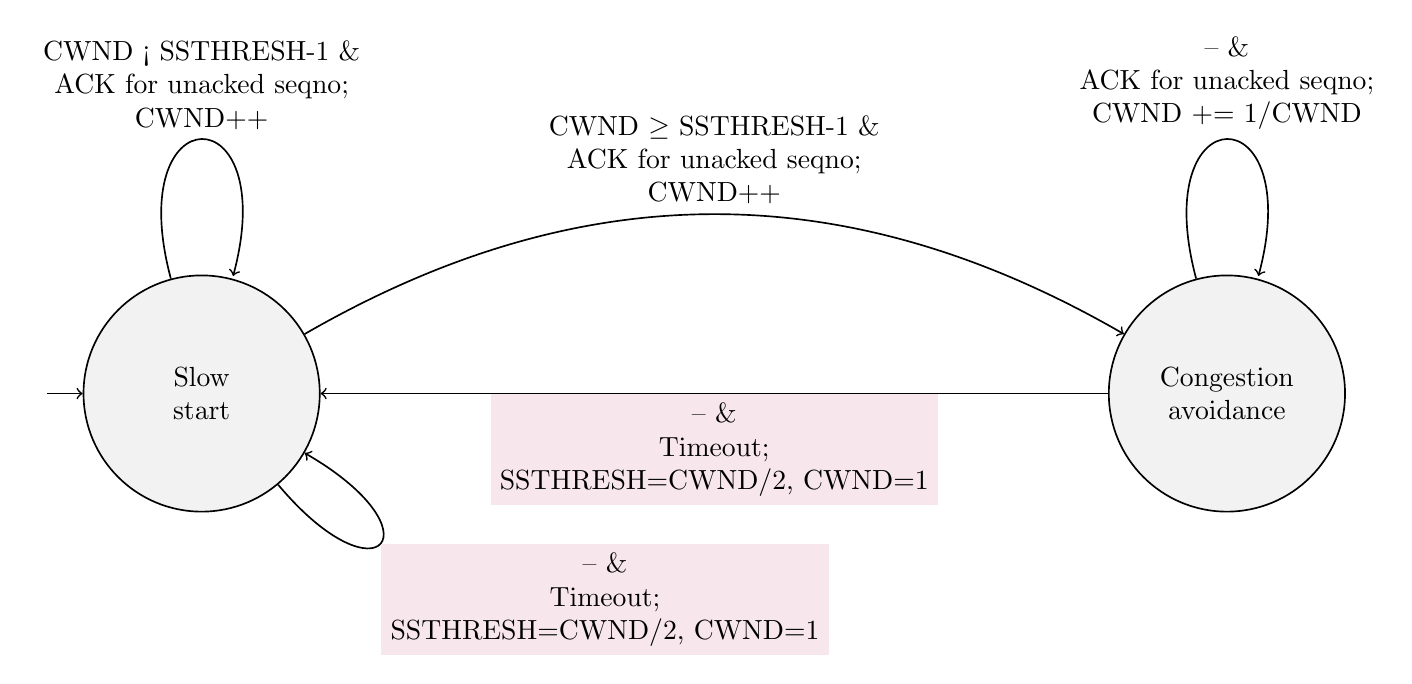
\begin{tikzpicture}[bend angle=30]
  \label{page:cc:tahoe_fsm}

  \node [state, initial, minimum width=3cm] (ss) {Slow\\ start};
  \node [state, minimum width=3cm, right=10cm of ss] (ca) {Congestion\\ avoidance};

  % ACK of previously unacked data:
  
  \draw (ss) edge [loop above] node [above]  {
    CWND < SSTHRESH-1 \& \\
    ACK for unacked seqno; \\
    CWND++
  } (ss); 

  \draw (ss) edge [bend left] node [above]  {
    CWND $\geq$ SSTHRESH-1 \& \\
    ACK for unacked seqno; \\
    CWND++
  } (ca); 
  
  \draw (ca) edge [loop above] node [above]  {
    --  \& \\
    ACK for unacked seqno; \\
    CWND += 1/CWND
  } (ca); 

  
  
  % timeout 
  \draw (ca) edge  node [below, fill=hpired!10 ] {
    --  \& \\
    Timeout; \\
    SSTHRESH=CWND/2, CWND=1
  } (ss);


  \draw (ss) edge [out=310, in=330, min distance=2cm] node [below right=0, fill=hpired!10] {
    --  \& \\
    Timeout; \\
    SSTHRESH=CWND/2, CWND=1
  } (ss);

  
\end{tikzpicture}


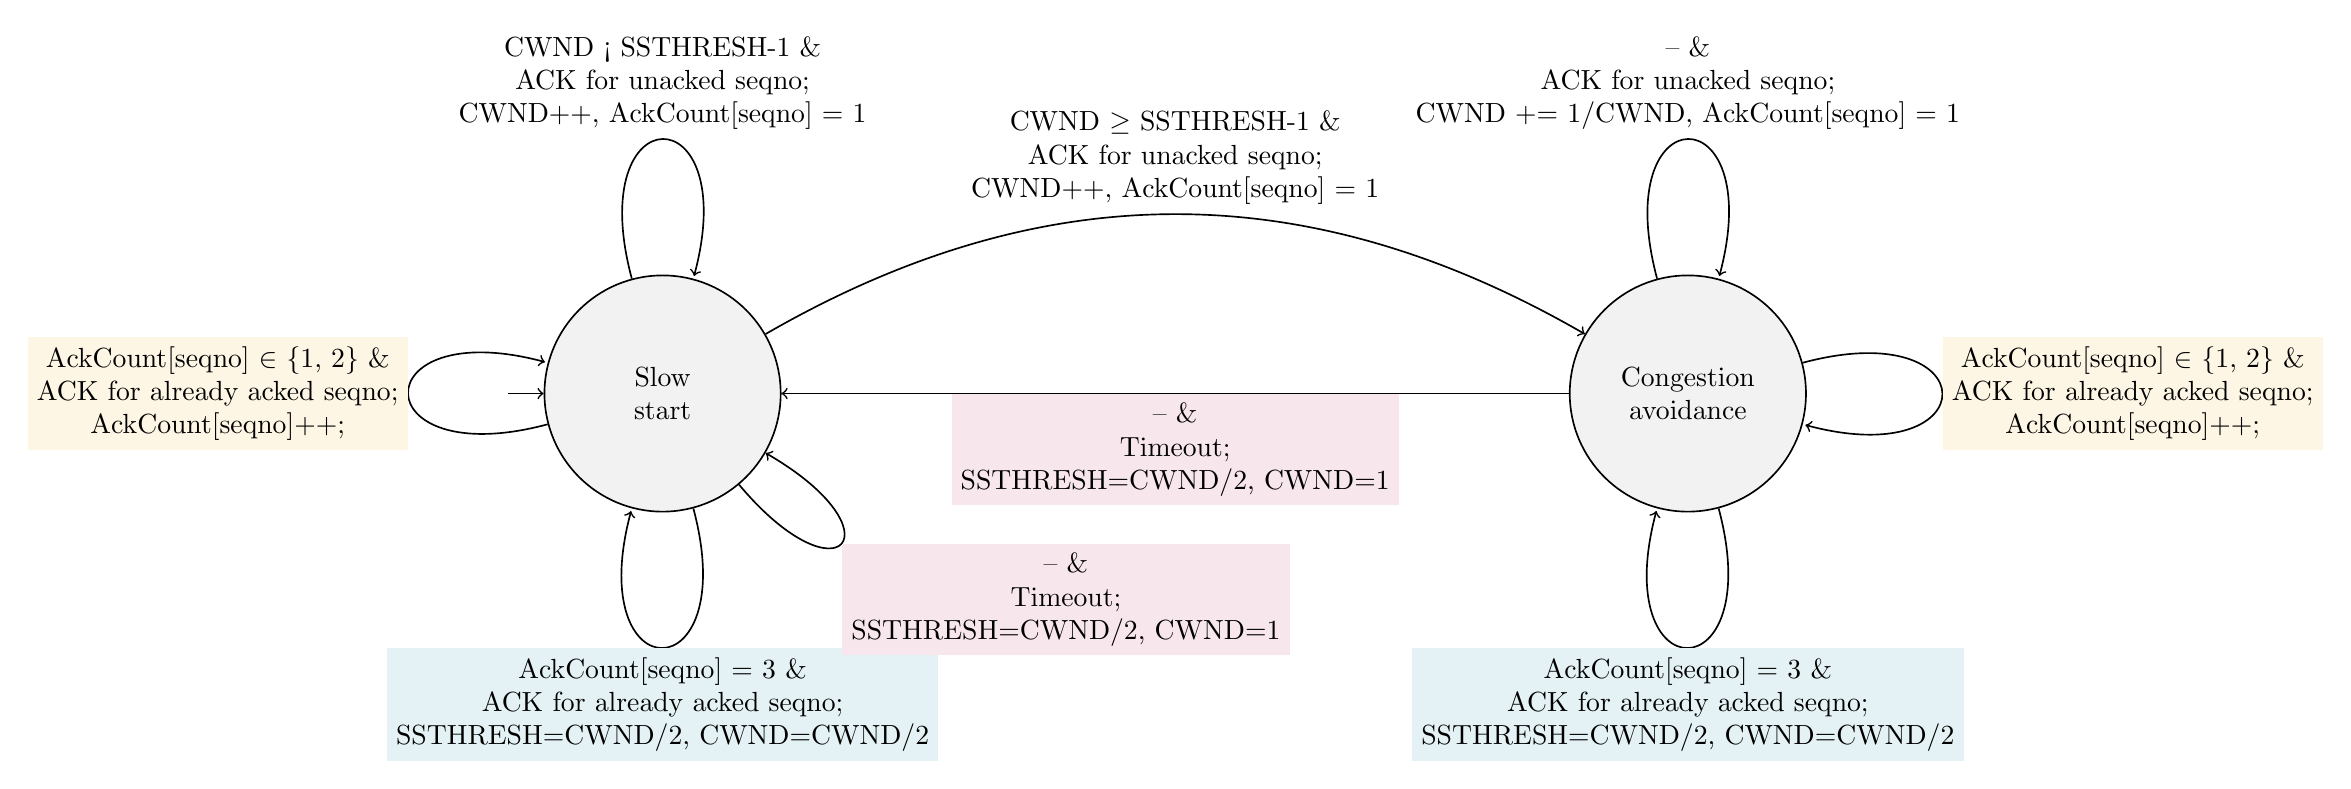
\begin{tikzpicture}[bend angle=30]
  \label{page:cc:reno_fsm}

  \node [state, initial, minimum width=3cm] (ss) {Slow\\ start};
  \node [state, minimum width=3cm, right=10cm of ss] (ca) {Congestion\\ avoidance};

  % ACK of previously unacked data:
  
  \draw (ss) edge [loop above] node [above]  {
    CWND < SSTHRESH-1 \& \\
    ACK for unacked seqno; \\
    CWND++, AckCount[seqno]  = 1
  } (ss); 

  \draw (ss) edge [bend left] node [above]  {
    CWND $\geq$ SSTHRESH-1 \& \\
    ACK for unacked seqno; \\
    CWND++, AckCount[seqno]  = 1
  } (ca); 
  
  \draw (ca) edge [loop above] node [above]  {
    --  \& \\
    ACK for unacked seqno; \\
    CWND += 1/CWND, AckCount[seqno]  = 1
  } (ca); 

  % dupack reveived, but not yet number three

  \draw (ss) edge [loop left] node [left, fill=hpiyellow!10] {
    AckCount[seqno] $\in$ \{1, 2\} \& \\
    ACK for already acked seqno; \\
    AckCount[seqno]++; 
  } (ss);

  \draw (ca) edge [loop right] node [right, fill=hpiyellow!10] {
    AckCount[seqno] $\in$ \{1, 2\} \& \\
    ACK for already acked seqno; \\
    AckCount[seqno]++; 
  } (ca);


  % third dupack received: 
  \draw (ss) edge [loop below] node [below, fill=hpiblue!10] {
    AckCount[seqno] = 3 \& \\
    ACK for already acked seqno; \\
    SSTHRESH=CWND/2, CWND=CWND/2
  } (ss);

  \draw (ca) edge [loop below] node [below, fill=hpiblue!10] {
    AckCount[seqno] = 3 \& \\
    ACK for already acked seqno; \\
    SSTHRESH=CWND/2, CWND=CWND/2
  } (ca);
  
  
  % timeout 
  \draw (ca) edge  node [below, fill=hpired!10 ] {
    --  \& \\
    Timeout; \\
    SSTHRESH=CWND/2, CWND=1
  } (ss);


  \draw (ss) edge [out=310, in=330, min distance=2cm] node [below right=0, fill=hpired!10] {
    --  \& \\
    Timeout; \\
    SSTHRESH=CWND/2, CWND=1
  } (ss);

  
\end{tikzpicture}

\end{document}



